\documentclass{article}
\usepackage[utf8]{inputenc}
\usepackage{parskip}

\usepackage{graphicx}
\graphicspath{ {images/} }

\usepackage{listings}
\usepackage{color}

\definecolor{dkgreen}{rgb}{0,0.6,0}
\definecolor{gray}{rgb}{0.5,0.5,0.5}
\definecolor{mauve}{rgb}{0.58,0,0.82}

\lstset{frame=tb,
	language=Java,
	aboveskip=3mm,
	belowskip=3mm,
	showstringspaces=false,
	columns=flexible,
	basicstyle={\small\ttfamily},
	numbers=none,
	numberstyle=\tiny\color{gray},
	keywordstyle=\color{blue},
	commentstyle=\color{dkgreen},
	stringstyle=\color{mauve},
	breaklines=true,
	breakatwhitespace=true,
	tabsize=3
}


\begin{document}
	\begin{titlepage}
		\begin{center}
			\textsc{\Large  Eötvös Loránd Tudományegyetem}
			\textsc{\Large  Informatikai Kar} \\
			[6cm]
			\huge{\bfseries Petz Dávid}
			
			\huge{\bfseries Szakdolgozat}
			
			\huge{\bfseries Maven és Gradle függőségek átalakítása} \\
			[6cm]
			
			\begin{flushright}
				\textsc{\large Témavezető: }
				
				\textsc{\large Horváth Gábor}
			\end{flushright}			
		\end{center}
	\end{titlepage}
	\newpage
	\tableofcontents
	\newpage
	\section{Nyilatkozatok}\label{sec:statement}
	\begin{center}
		Elfogadási nyilatkozat
	\end{center}
	Ezen tervezési feladat az Eötvös Loránd Tudományegyetem Fordítóprogramok Tanszék által a Szakdolgozat feladatokra előírt valamennyi tartalmi és formai követelménynek maradéktalanul eleget tesz. E tervezési feladatot a nyilvános bírálatra és nyilvános előadásra alkalmasnak tartom.
	
	A beadás időpontja: \\
	[0.2cm]
	
	\begin{flushright}
		Témavezető
	\end{flushright}  
	\begin{center}
		Nyilatkozat az önálló munkáról
	\end{center}
	Alulírott, Petz Dávid (CB1X9V), az Eötvös Loránd Tudományegyetem hallgatója, büntetőjogi és fegyelmi felelősségem tudatában kijelentem és sajátkezű aláírásommal igazolom, hogy ezt a szakdolgozatot meg nem engedett segítség nélkül, saját magam készítettem, és a szakdolgozat feladatomban csak a megadott forrásokat használtam fel. Minden olyan részt, melyet szó szerint vagy azonos értelemben, de átfogalmazva más forrásból átvettem, egyértelműen, a forrás megadásával megjelöltem. \\
	[0.2cm]
	\begin{flushright}
		Hallgató
	\end{flushright}

	\newpage
	
	\section{Előszó}\label{sec:prolog}
	A választásom azért esett erre a témára mert mindig is érdekeltek a Java fejlesztést megkönnyítő eszközök használata. Továbbá mindennapi munkám során dolgozom ezen két technológiával, viszont egy problémára sosem találtam kielégítendő megoldást.
	
	Azóta amióta dolgozom ezen eszközökkel sokszor felmerült az a probléma, hogy hogyan lehet biztosítani az átjárást a két eszköz között, viszont nem találtam kutatásaim során pontos választ erre a kérdésre. Sokszor csak félig kész vagy hibás megoldásokat találtam így elhatároztam, hogy ezen dolgozat témájaként fogom orvosolni a jelenlévő problémát.
	
	A feladat elkészítése során ügyeltem arra, hogy a kiírásban megadott szempontoknak minél alaposabban eleget tegyek.
	
	Külön köszönet konzulensemnek, Horváth Gábornak, aki tanácsaival hozzájárult a dolgozatom elkészítéséhez.
	
	\newpage
	\section{Bevezetés}\label{sec:introduction}
	\subsection{Célkitűzések}\label{subsec:goals}
	A projekt management eszközök igen fontos szerepet játszanak a Java projektek fejlesztése során. Különböző feladatokat szerveznek egybe és egyesítenek. Például lefuttatják a teszteket, lefordítják a kódot, kódelemzőket futtatnak a forráskódon, így leveszik ezeknek a terhét a fejlesztők válláról. 
	\subsection{Áttekintés}\label{subsec:review}
	asdsa
	\newpage
\section{Szakirodalmi áttekintés}\label{sec:prof_review}
A lent ismertetésre kerülő technológiák mindegyikét felhasználtam a dolgozat elkészítéséhez. Első sorban a könyvtár fejlesztéséhez használt módszerek kerülnek ismertetésre néhány alapfogalom mellett, majd a könyvtár használatának szemléltetéséhez elkészült webes felület.
\subsection{Projekt management eszköz}\label{subsec:project_management_tool}
A Java fejlesztés világának szerves részeit képezik ezen eszközök. A legnagyobb erejük abban rejlik, hogy olyan lépéseket automatizálnak melyek egy fejlesztés során nagyon gyakran előfordulnak. Például a teszteket lefuttatása, projekt fordítása vagy a függőségek kezelése. Úgy teszik ezt lehetővé, hogy minden ilyen eszközhöz tartozik egy konfigurációs fájl amiben előre vannak definiálva a projektre jellemző adatok. Ezen adatokat a fejlesztőknek kell megadni egyszer és tetszőlegesen módosíthatják a projekt élettartama alatt. Ezek után már csak a rendszer által használt parancsokat kell futtatniuk.
\subsection{Apache Ant}\label{subsec:ant}
Ezen rendszer megjelenése a 2000-es évek elejére tehető. Ez volt az első jelentős eszköz a Java nyelvhez. A Unixos Make rendszer volt a kiindulási pont, viszont a legfontosabb különbség az volt, hogy az Ant XML fájlt használ a konfiguráláshoz. A lenti forráskód egy példa konfigurációt mutat:
\lstset{
	language=XML,
	morekeywords={encoding,
		xs:schema,xs:element,xs:complexType,xs:sequence,xs:attribute}
}
\begin{lstlisting}
<?xml version="1.0"?>
<project name="Hello" default="compile">
<target name="clean" description="remove intermediate files">
<delete dir="classes"/>
</target>
<target name="clobber" depends="clean" description="remove all artifact files">
<delete file="hello.jar"/>
</target>
<target name="compile" description="compile the Java source code to class files">
<mkdir dir="classes"/>
<javac srcdir="." destdir="classes"/>
</target>
<target name="jar" depends="compile" description="create a Jar file for the application">
<jar destfile="hello.jar">
<fileset dir="classes" includes="**/*.class"/>
<manifest>
<attribute name="Main-Class" value="HelloProgram"/>
</manifest>
</jar>
</target>
</project>
\end{lstlisting}
Azonban ennek az volt a hátránya, hogy nagyobb projektek esetén hatalmas XML fájlokkal kellett dolgozni. Mára az Ant csak legacy projekteken fordul elő, helyét átvette a Maven és Gradle.
\subsection{Apache Maven}\label{subsec:maven}
Az Apache Maven 2002-ben készítette el Jason van Zyl. Felépítésében és használatában nagyon hasonlít az Apache Ant-ra azonban bevezet egy új fogalmat: POM (angolul: Project Object Model). POM a fordítandó projektet írja le és annak függőségeit. Az egyes lépéseket céloknak (angolul: goal) nevezzük:
\begin{itemize}
	\item validate: Ellenőrzi a projekt beállításait.
	\item compile: Lefordítja a forráskódokat
	\item test: Lefuttatja a teszteket
	\item package: Becsomagolja a forráskódokat a megadott formátumba. Például jar.
	\item verify: 
	\item install: Berakja a csomagot a lokális repository-ba.
	\item deploy: A fordítás végén beküldi a távoli repository-ba.
\end{itemize}
Egy példa a pom.xml fájlra:
\lstset{
	language=XML,
	morekeywords={encoding,
		xs:schema,xs:element,xs:complexType,xs:sequence,xs:attribute}
}
\begin{lstlisting}
<project>
	<modelVersion>4.0.0</modelVersion>
	<groupId>com.mycompany.app</groupId>
	<artifactId>my-app</artifactId>
	<version>1.0</version>
	<dependencies>
		<dependency>
			<groupId>junit</groupId>
			<artifactId>junit</artifactId>
			<version>3.8.1</version>
			<scope>test</scope>
		</dependency>
	</dependencies>
</project>
\end{lstlisting}
Az eszköz használata terminálból történik. A projekt gyökér könyvtárából kell kiadni a célok neveit egy "mvn" kulcsszóval megelőzve. Fontos megjegyezni, hogy lehet őket kombinálni. Íme egy gyakorlati példa:
\begin{lstlisting}[language=bash]
$ mvn clean package
\end{lstlisting}
Ezt a parancsot futtatva a következő kimenetet kapjuk egy sikeres fordítása esetben: 
\begin{lstlisting}
[INFO] ----------------------------------------------------------------------------
[INFO] Building Maven Quick Start Archetype
[INFO]    task-segment: [compile]
[INFO] ----------------------------------------------------------------------------
[INFO] artifact org.apache.maven.plugins:maven-resources-plugin: \
checking for updates from central
...
[INFO] artifact org.apache.maven.plugins:maven-compiler-plugin: \
checking for updates from central
...
[INFO] [resources:resources]
...
[INFO] [compiler:compile]
Compiling 1 source file to <dir>/my-app/target/classes
[INFO] ----------------------------------------------------------------------------
[INFO] BUILD SUCCESSFUL
[INFO] ----------------------------------------------------------------------------
[INFO] Total time: 3 minutes 54 seconds
[INFO] Finished at: Sat March 10 15:48:34 GMT-05:00 2018
[INFO] Final Memory: 2M/6M
[INFO] ----------------------------------------------------------------------------
\end{lstlisting}
\subsection{Függőség}\label{subsec:dependency}
Ide jön a defi.

A függőségeket különböző attribútumokkal tudjuk leírni és ezeket használjuk a Gradle és Maven esetében amikor importálni szeretnék őket a projektünkbe. Importálás során az úgy nevezett CLASSPATH változóba írodnak bele ezeket az adatok és a fejlesztői környezetek innen olvassák ki, hogy hol keressék a függőségeket. A függőségeket leíró adatok:
\begin{itemize}
	\item groupId: A függőséget tartalmazó csomag megnevezése. Például: com.test
	\item artifactId: A függőség neve. Például: test
	\item version: A függőség verziója. Adott függőségből egy újabb kiadás magasabb verziószámú. Például: 1.0.1
	\item scope: A függőségeknek 6 lehetséges láthatóságát (angolul: scope) különböztetjük meg:
	\begin{itemize}
		\item complie: Ha nem adunk meg semmilyen láthatóságot a függőségnek akkor ez lesz az alapértelmezett érték.
		\item provided: Hasonlít a complile láthatósághoz viszont itt azt feltételezi a rendszer, hogy valahol már megvan ez a függőség (például: JDK vagy a futtatási környezet adja). Nem tranzitív. 
		\item runtime: Nem szükséges a fordításhoz csak a futtatáshoz.
		\item test: Az alkalmazás működéséhez nem szükséges csak a teszteléséhez. Nem tranzitív.
		\item system: Hasonlít a provided láthatósághoz viszont itt a függőségeket kezelő rendszer nem fogja keresni az adott függőséget egy repository-ban sem, a fejlesztőnek kell biztosítani kívülről a meglétét.
		\item import: 
	\end{itemize}
\end{itemize}
Így a fenti attribútumok alapján egy Maven-es függőség a következőképpen jön létre:
\begin{lstlisting}
<dependency>
	<groupId>junit</groupId>
	<artifactId>junit</artifactId>
	<version>3.8.1</version>
	<scope>test</scope>
</dependency>
\end{lstlisting}
\subsection{Repository}\label{subsec:repo}
Mivel a Maven és Gradle hálózatképes így szükség esetén le tudják tölteni a különböző komponenseket távoli szervergépekről. Ezeket a komponenseket úgy nevezett Repository-ban tárolják ahová fel és le is lehet tölteni függőségeket. Három fajta repository típust különböztetünk meg: 
\begin{itemize}
	\item Lokális: A fejlesztői számítógépen tárolódik egy .m2 nevű rejtett mappában. A mappa elérési útja függ a használt operációs rendszertől. Itt tárolja a fejlesztés során használt függőségeket. Ha itt nem található meg a kért függőség akkor a Távoli repository-ból ide tölti és tárolja le azt későbbi használatra.
	\item Távoli: Röviden "Maven Central". Itt tárolódik el az összes létező függőség amit elkészítettek a Maven rendszerhez, melyet az Apache felügyel. Jelenleg több ezer könyvtár található itt és napi szinten kerülnek bele új komponensek. Böngészőből könnyen elérhetjük mi is a https://search.maven.org/ oldalon. Fontos megjegyezni, hogy a Gradle is innen tölti le a függőségeket.
	\item Nexus: Vállalatok számára nyújt belső tárolási lehetőséget. Lényegében ugyan olyan mint a Távoli viszont ebben az esetben a felügyeleti jog az üzemeltető vállalaté. Biztonságkritikus projektek estében le szokták tiltani a Maven Centralt és az itt található függőségekből dolgoznak a fejlesztők, mivel könyvtárakat a cég szakemberei ellenőrizték. Jellemzően egy Linuxos szervergépre szokták feltelepíteni.
\end{itemize}
\subsection{Gradle}\label{subsec:gradle}
A Gradle egy nyílt forráskodú projektént indult még 2007-ben, melyben az Apache Ant és Maven koncepcióit vették alapul a fejlesztők, azonban eltértek az XML alapú kezeléstől és egy Groovy alapú DSL (angolul: domain-specific-language) megvalósítást választottak. Erre példát itt láthatunk: 
\begin{lstlisting}
apply plugin: 'java'
apply plugin: 'eclipse'

sourceCompatibility = 1.7
version = '1.0'
jar {
	manifest {
		attributes 'Implementation-Title': 'Gradle Quickstart',
		'Implementation-Version': version
	}
}

repositories {
	mavenCentral()
}

dependencies {
	compile group: 'commons-collections', name: 'commons-collections', version: '3.2.2'
	testCompile group: 'junit', name: 'junit', version: '4.+'
}

test {
	systemProperties 'property': 'value'
}

uploadArchives {
	repositories {
	flatDir {
		dirs 'repos'
		}
	}
}
\end{lstlisting}
Használata nem tér el a Maven megközelítésétől, szintén terminálból kell kiadni a parancsokat a projekt gyökér könyvtárából. Ha lefuttatjuk egy gradle projektre a következő parancsot:
\begin{lstlisting}[language=bash]
$ gradle build
\end{lstlisting}
Akkor ez a kimenet meg fog megjelenni egy sikeres fordítás után:
\begin{lstlisting}[language=bash]
:compileJava
:processResources
:classes
:jar
:assemble
:compileTestJava
:processTestResources
:testClasses
:test
:check
:build

BUILD SUCCESSFUL
\end{lstlisting}
\subsection{Java Servlet Container}\label{subsec:java_servlet}
A servlet konténer (angolul: web container vagy servlet container) egy olyan komponense egy web szervernek amely Java servletekkel kommunikál. A konténer felelős igen széleskörű, néhány fontosabb ezek közül:
\begin{itemize}
	\item Alkalmazások életciklusának kezelése
	\item Szálkezelés
	\item HTTP kérések továbbítása a megfelelő servlet-nek
	\item Tranzakció kezelés
	\item Biztonság
\end{itemize} 
\begin{center}
	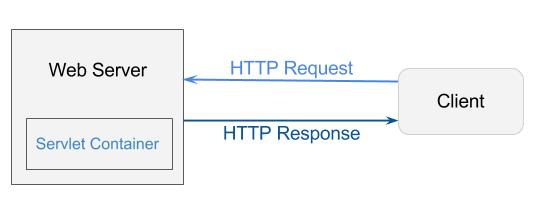
\includegraphics[width=10cm, height=6cm]{web-server-servlet-container}
	
	A fenti képen a servlet működése látható röviden.
\end{center}

Mint a képen is látható a servlet konténer nem más mint servletek gyűjteménye, amiket egy webszerver kezel. Ezt a technológiát legegyszerűbben úgy lehet leírni, mint egy interface-t melynek több megvalósítása létezik. Az alábbi listában a legelterjedtebb implementációkat láthatjuk: 
\begin{itemize}
	\item Apache Tomcat
	\item Jetty
	\item Glassfish
	\item WebLogic Application Server
\end{itemize}
Üzemeltetésük úgy történik, hogy egy szervergépen futtatják valamely megvalósítását a konténernek amely futtatni fogja a webes alkalmazásunkat.

A dolgozatban az Apache Tomcat-et használtam.

\subsection{Apache Tomcat}\label{subsec:tomcat}
Az Apache Tomcat vagy másik nevén "Tomcat szerver" egy nyílt forráskódú, ingyenes Java Servlet Container melyet az Apache fejlesztett a 90-es évek végén. Feladata a különböző webes alkalmazások futtatása. Ezen művelet úgy történik, hogy Maven vagy Gradle megkapja a webes alkalmazásunk Java, Javascript forráskódját, HTMl és CSS kódokat majd egy speciális WAR (Web application Archive) fájlt készít belőlük amit a Tomcat már képes kezelni. Az elkészült WAR fált ezek után elindítja (deployolja) az előre megadott elérési útra. A Tomcat kezelése történhet a fejlesztői környezetből vagy a böngészőben futó kezelőfelületről is.

\begin{center}
	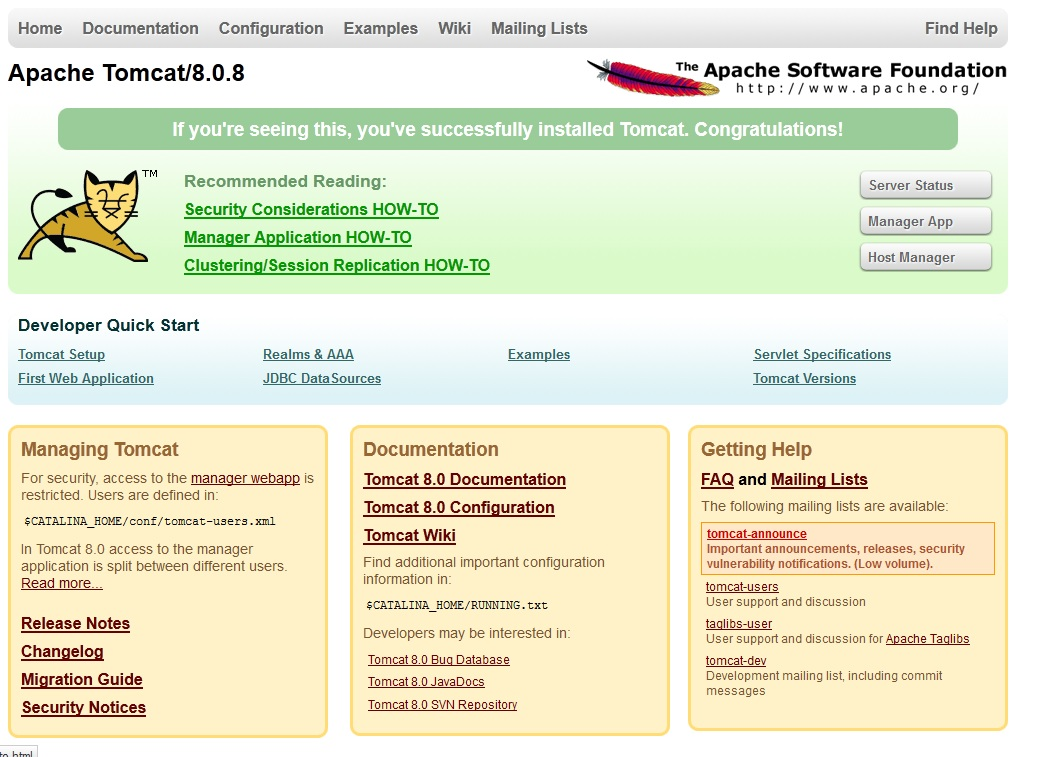
\includegraphics[width=10cm, height=6cm]{tomcat_settings}
	
	A fenti képen látható a böngészőből elérhető felület.
\end{center}


\subsection{Streaming API for XML (StAX)}\label{subsec:stax}
Az XML fájlformátum kezelésére több API is létezik a Java-ban, az alábbi táblázatban található róluk egy kisebb összefoglaló:
\begin{center}
	\begin{tabular}{ | l | l | l | l | }
		\hline
		Feature & StaX & SAX & DOM \\
		\hline
		API Type & Pull, streaming & Push,streaming & In memory tree \\
		Ease of Use & High & Medium & High \\
		XPath Capability & No & No & Yes \\
		CPU/memory Efficiency & Good & Good & Varies \\
		Random access & Yes & Yes & Yes \\
		Read XMl & Yes & Yes & Yes \\
		Write XML & Yes & No & Yes \\
		CRUD & No & No & No \\
		\hline
	\end{tabular}
\end{center}
Mint a táblázatból is kiderül, kettő féle képen lehet beolvasni XMl fájlokat. Az egyik megközelítés az, hogy a memóriában tároljuk a teljes fát, a másik pedig folytonos olvasás. Mivel nagyobb fáljok esetén a fa tárolása túl költséges művelet lehet így folytonos olvasás módszere mellett döntöttem. Erre a StaX és SAX könyvtárak megfelelőek, viszont utóbbi keretrendszer csak olvasni tud fájlokat, írni már nem. Így végül a StaX könyvtár mellett döntöttem.
\subsection{Spring Framework}\label{subsec:spring}
A Spring egy nyílt forráskódú keretrendszer a Java nyelvhez mely az "inversion of control" filozófiát valósítja meg. Leginkább webes alkalmazások fejlesztésben használják, továbbá az EJB (Enterprise JavaBean) modellt helyettesíti. A Spring nem egy nagy keretrendszer hanem sok kisebb méretű modulok együttes használatát teszi lehetővé. Néhány elterjedt modul:
\begin{itemize}
	\item Spring Core
	\item Spring AOP
	\item Spring Security
	\item Spring MVC
	\item Spring Data
\end{itemize}
A másik nagyon fontos fogalom a Spring esetében a Bean kifejezés. Egy többrétegű alkalmazás esetében a különböző rétegeknek kommunikálni kell egymással és ezt úgy lehet elérni a Springes világban, hogy ezen rétegeket bean-enként definiáljuk. A definiális kettő féle képpen történhet, külön XML fájlba definiáljuk a bean-eket vagy úgy nevezett Java config fájlban példányosítjuk egy @Bean annotációval ellátva, majd a megfelelő osztályban egy @Autowired annotációval definiáljuk a referenciát és a Spring az alkalmazás indulásakkor példányosítja a referenciákat. A lenti képeken látható egy-egy példa.

XML-es bean definíció:
\begin{lstlisting}
<?xml version="1.0" encoding="UTF-8"?>
<beans xmlns="http://www.springframework.org/schema/beans"
xmlns:xsi="http://www.w3.org/2001/XMLSchema-instance"
xsi:schemaLocation="http://www.springframework.org/schema/beans
http://www.springframework.org/schema/beans/spring-beans.xsd">

<!-- services -->

<bean id="petStore" 
class="org.springframework.samples.jpetstore.services.PetStoreService">
	<property name="accountDao" ref="accountDao"/>
	<property name="itemDao" ref="itemDao"/>
</bean>

<!-- more bean definitions for services go here -->

</beans>
\end{lstlisting}

Java-s konfigurációs osztály. Ezt fogja a Spring beolvasni a Bean-ek létrehozásához. 
\begin{lstlisting}
@Configuration
public class AppConfig {
	@Bean
	public ItemDao itemDao() {
		return new ItemDao();
	}
	@Bean
	public AccountDao accountDao() {
		return new AccountDao();
	}
	@Bean
	public PetStoreService petStoreService() {
		return new PetStoreService();
	}
}
\end{lstlisting}
A PetStoreService osztály forráskódja:
\begin{lstlisting}
public class PetStoreService {
	@Autowired
	private AccountDao accountDao;
	@Autowired
	private ItemDao itemDao;
	
	...
}
\end{lstlisting}
Ezek után a két @Autowired annotációval ellátot referenciát létrehozza a Spring.

Az XML-es változat még a régebbi konvenciókat követi, legacy projekteken még megtaláló ez a fajta konfiguráció, újabban a Java-s megoldást választják a fejlesztők, mivel Java forráskódú a definiálás is így lehetőségük van alkalmazni a Dependency Injection módszert. A dolgozatban Java-s bean definíciókat használtam.

\subsection{Boostrap}\label{subsec:boostrap}
Twitter fejlesztésű nyílt forrású, ingyenes front-end keretrendszer melyben előre definiált CSS és HTMl szabályokat találunk, mint például formok, gombok, navigáció és némi Javascript bővítményt is tartalmaz. Mivel előre definiált szabályokat kell újra felhasználni, így nagyban gyorsítja egy felület kifejlesztését. Fontos megjegyezni, hogy ez csak front-end fejlesztésre használható könyvtár. 

\begin{center}
	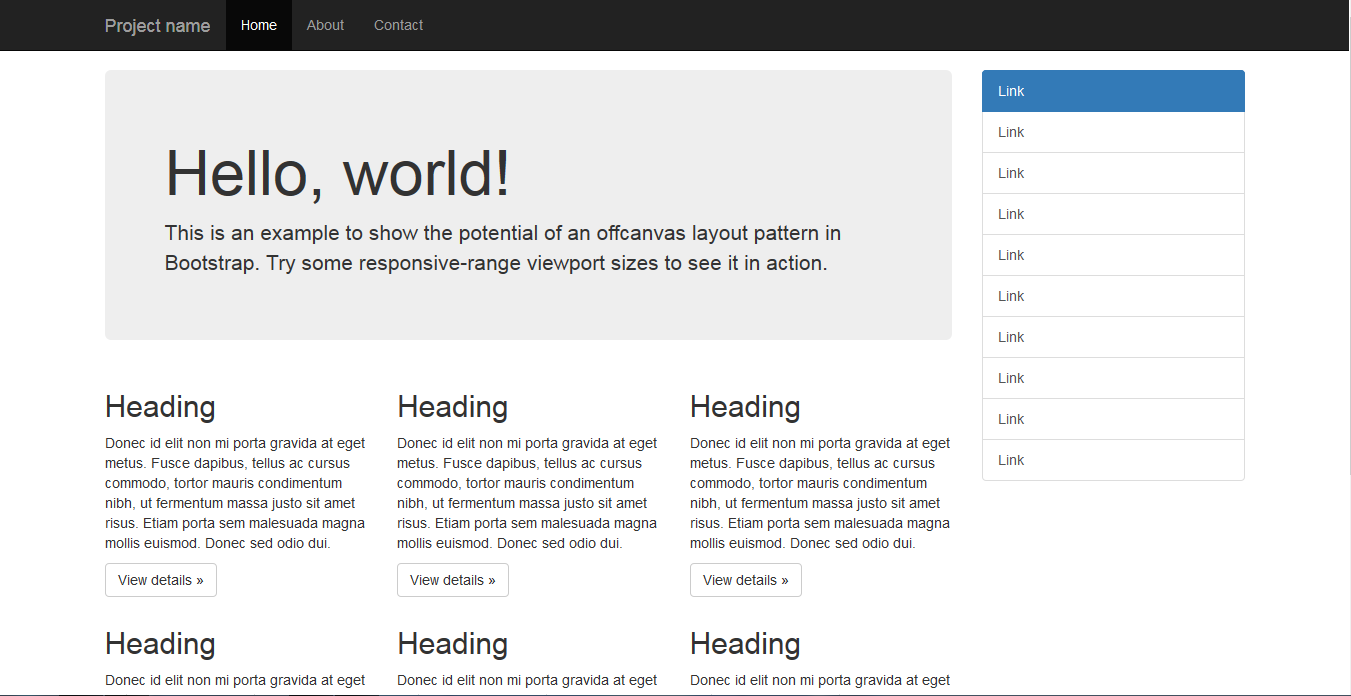
\includegraphics[width=10cm, height=6cm]{boostrap_example}
	
	A fenti képen egy Bootstrapes példa oldal látható.
\end{center}
	A szakdolgozat könytár részét demonstráló webes felület kinézetéért ezen technológia a felelős.
\end{document}